\subsection{Unified Modellig Language}
En af de anvendte sprog indenfor objektorienteret programmering er standarden Unified Modelling Language (UML). Ud fra denne standard anvendes modeller til at visualisere struktur og egenskaber af systemet. Derudover relaterer metoderne til analyse og design af systemet. Til visualiseringen anvendes forskellige UML diagrammer som kan opdeles i tre kategorier, herunder adfærds-, struktur- og interaktiondiagrammer.  Adfærdsdiagrammer er for eksempel use case- og  aktivitetsdiagram, mens strukturdiagrammer kan være klassediagrammer og interaktionsdiagrammer kan være sekvensdiagrammer. \cite{Fowler2004, Williams2004}.


\subsubsection{Use case diagrammer} 
Use case diagrammer benyttes til at illustrere aktørernes interaktion med et system samt, hvordan forskellige use cases interagerer mellem hinanden. Dertil er use case diagrammet med til at repræsentere funktionelle krav for systemet. \cite{Williams2004} Et eksempel på et use case diagram ses af \autoref{fig:use_case}.

\begin{figure} [H]
\centering
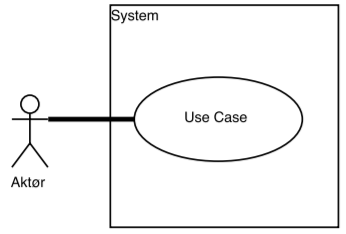
\includegraphics[width=0.5\textwidth]{figures/USE_CASE2}
\caption{Simpelt use case diagram.}
\label{fig:use_case}
\end{figure}

\noindent
Af \autoref{fig:use_case} ses aktørens interaktion med use case visualiseret som en streg mellem de to. I et use case diagram vil aktøren definere en person, der kan tilgå systemets funktionaliteter. Dette kan eksempelvis være en person, rolle, objekt eller en anden given genstand. Hertil vil den enkelte use case beskrive en handling eller funktionalitet i systemet. Ved anvendelse af flere use cases kan der opstå et forhold mellem de enkelte use cases. Dette forhold visualiseres med en stiblet pil mellem use casene og kan enten være include eller extend. Hvis en use case ikke kan stå alene og derfor er nødt til at arve noget fra en anden use case er denne include. Modsat kan extend anvendes, hvis use casen kan stå alene. \cite{Fowler2004, Williams2004}


\subsubsection{Aktivitetsdiagrammer} 
Aktivitetsdiagrammer anvendes til at beskrive, hvad der sker i programmet, herunder proceduremæssig logik, business processer og arbejdsflow. Aktiviteter kan opdeles i subaktiviteter eller metoder. Subaktiviteter vil fremgå af diagrammet ved et rivesymbol, mens metoder vil fremgå ved syntaksen klasse-navn::metode-navn. Aktivitetsdiagrammer fortæller ikke, hvem der udfører aktiviteten, hertil kan der anvendes skillevægge, som viser, hvilken aktivitet en klasse eller organisation tilhører. For at holde et aktivitetsdiagram enkelt kan der anvendes et brillesymbol i en aktivitet. Denne aktivitet vil efterfølgende kunne beskrives yderligere i et nyt aktivitetsdiagram.\cite{Fowler2004} Symboler, der kan anvendes inden for aktivitetsdiagrammer, fremgår af \autoref{fig:aktivitetsdiagram}.

\begin{figure} [H]
\centering
\includegraphics[width=0.9\textwidth]{figures/aktivitetsdiagram}
\caption{Symboler der kan anvendes i aktivitetsdiagrammer. Revideret \cite{Fowler2004}.}
\label{fig:aktivitetsdiagram}
\end{figure}


%Til at beskrive komplekse use cases eller klassemetoder anvendes aktivitetsdiagrammer. Dette giver overblik over flowet gennem de forskellige aktiviteter i den givne funktion eller metode. \cite{Fowler2004}    

%Såfremt der i et aktivitetsdiagram anvendes et 'brille' symbol, indikerer dette at den aktivitet i sig selv er kompleks og er beskrevet i et særskilt aktivitetsdiagram.  

\subsubsection{Klassediagrammer}
Klassediagrammer anvendes som redskab til at beskrive strukturen i et givent system og dermed skabe overblik over forskellige klasser og relationer, der indgår i systemet \cite{Fowler2004}. Det fremgår af \autoref{fig:klassediagram}, at hver klasse identificeres ud fra et unikt klassenavn, hvor der yderligere kan tildeles attributter og metoder til klassen.

\begin{figure} [H]
\centering
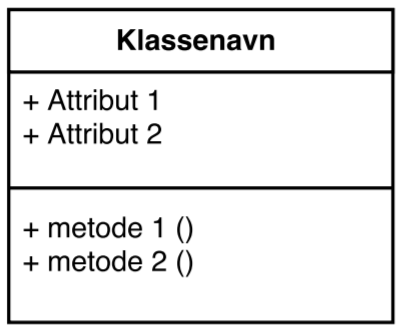
\includegraphics[width=0.3\textwidth]{figures/klassediag}
\caption{I klassediagrammer identificeres klasser ud fra et klassenavn, og dertilhørende attributter og metoder tilføjes nedenfor navnet. Revideret \cite{Fowler2004}.}
\label{fig:klassediagram}
\end{figure}

\noindent
Attributter og metoder kan markeres med symbolerne; +, - eller \#, som symboliserer, at de henholdsvis er public, private eller beskyttede, jf. \autoref{sec:OOP}.

Relationerne mellem klasserne illustreres ved brug af forskellige pile, og disse kan navngives for at tydeliggøre forholdet mellem  klasserne. Yderligere kan multipliciteten angives ved at tilføje symbolet *, der angiver "mange", eller specifikke værdier i pilenes ender. 


\subsubsection{Sekvensdiagrammer}
Sekvensdiagrammer anvendes til at beskrive detaljer om, hvilke og hvornår forskellige operationer udføres. Disse diagrammer er organiseret efter tid. De forskellige objekter som anvendes i operationerne er angivet fra venstre mod højre. Sekvensdiagrammer anvendes i design og er udarbejdet ud fra use case diagrammer.\cite{Brahma2015} Et simpelt sekvensdiagram fremgår af \autoref{fig:sekvens}

\begin{figure} [H]
\centering
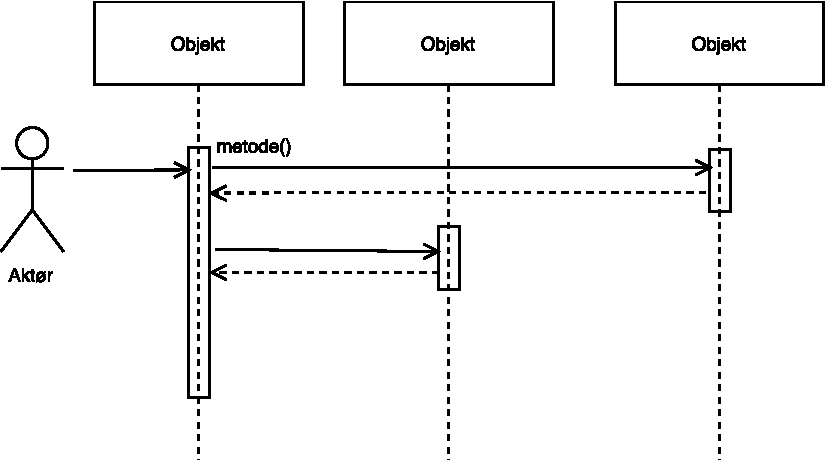
\includegraphics[width=0.3\textwidth]{figures/sekvens}
\caption{Simpelt sekvensdiagram. Revideret \cite{Brahma2015}.}
\label{fig:sekvens}
\end{figure}

\noindent
Hver entitet i use case diagrammet har en kolonne i sekvensdiagrammet. Den vertikale retning beskriver tiden og de horisontale linjer illustrerer funktionaliteter. For enden af de horisontale linjer er der navngivet metoden på entiteten. \cite{Brahma2015}